\documentclass[10pt]{article}
\usepackage[margin=0.8in]{geometry}
\usepackage[utf8]{inputenc}
\usepackage[T1]{fontenc}
\usepackage{graphicx}
\usepackage[export]{adjustbox}
\graphicspath{ {./diff_kinematics/} }
\usepackage{amsmath}
\usepackage{amsfonts}
\usepackage{amssymb}
\usepackage[version=4]{mhchem}
\usepackage{stmaryrd}
\usepackage{bbold}
\usepackage{fixltx2e}
\usepackage{caption}
\usepackage{mathtools}
\usepackage[parfill]{parskip}
\usepackage{float}

\begin{document}



\title{Lecture 10: Derivative of Transformation}
\date{Sep. 19, 2023}
\author{Wanxin Jin}
\maketitle




\section{Derivative of Rotation Matrix}

\noindent
Consider a time-varying rotation matrix $\boldsymbol{R}=\boldsymbol{R}(t)$. One has

$$
\boldsymbol{R}(t) \boldsymbol{R}^{T}(t)=\boldsymbol{I}
$$

Differentiating the above equation with respect to time gives

$$
\dot{\boldsymbol{R}}(t) \boldsymbol{R}^{T}(t)+\boldsymbol{R}(t) \dot{\boldsymbol{R}}^{T}(t)=\boldsymbol{S}(t)+\boldsymbol{S}^{T}(t)=\boldsymbol{O}
$$

with the newly defined $\boldsymbol{S}(t)=\dot{\boldsymbol{R}}(t) \boldsymbol{R}^{T}(t)$ being called a $(3 \times 3)$ skew-symmetric matrix, and 

$$
\dot{\boldsymbol{R}}(t)=\boldsymbol{S}(t) \boldsymbol{R}(t)
$$


Next, let's find the physical interpretation of $\boldsymbol{S}$.




Consider ${\boldsymbol{R}}(t)$ represents a rotation of a moving frame $O'-x'y'z'$ with respect to a fixed reference frame $O-xyz$. It means the following coordinate transformation
 $\boldsymbol{p}(t)=\boldsymbol{R}(t) \boldsymbol{p}^{\prime}$. Taking the derivative of both sides yields


$$
\dot{\boldsymbol{p}}(t)=\dot{\boldsymbol{R}}(t) \boldsymbol{p}^{\prime}=\boldsymbol{S}(t) \boldsymbol{R}(t) \boldsymbol{p}^{\prime}
$$

where we have used the defined skew-symmetric matrix $ \boldsymbol{S}(t)$, and  considered $\boldsymbol{p}^\prime$ is fixed in the moving  frame.

Recall that in the mechanics courses, given the angular velocity $\boldsymbol{\omega}(t)=\left[\begin{array}{lll}\omega_{x} & \omega_{y} & \omega_{z}\end{array}\right]^{T}$ of the moving frame  $O'-x'y'z'$, with respect to the fixed frame, we also write the derivative 
as

$$
\dot{\boldsymbol{p}}(t)=\boldsymbol{\omega}(t) \times \boldsymbol{R}(t) \boldsymbol{p}^{\prime}
$$

Comparing the above two equations, we can conclude

$$
\boldsymbol{S}=\left[\begin{array}{ccc}
0 & -\omega_{z} & \omega_{y} \\
\omega_{z} & 0 & -\omega_{x} \\
-\omega_{y} & \omega_{x} & 0
\end{array}\right]=\boldsymbol{S}(\boldsymbol{\omega})
$$

Hence, we can conclude the derivative of a rotation matrix is 
$$
\dot{\boldsymbol{R}}=\boldsymbol{S}(\boldsymbol{\omega}) \boldsymbol{R}$$


\emph{Note that in the above equation, $\boldsymbol{\omega}$ is expressed in the fixed frame.}


One property of $\boldsymbol{S}(\boldsymbol{\omega})$: if $\boldsymbol{R}$ denotes a rotation matrix, it can be shown that the following relation holds:

$$
    \boldsymbol{R} \boldsymbol{S}(\boldsymbol{\omega}) \boldsymbol{R}^{T}=\boldsymbol{S}(\boldsymbol{R} \boldsymbol{\omega})
$$

\section{Derivative of Pose Transformation}

Pose transformation defines coordinate mapping of a point $P$ from frame $O_1-x_1y_1z_1$ to frame $O_0-x_0y_0z_0$

$$
\boldsymbol{p}^{0}=\boldsymbol{o}_{1}^{0}+\boldsymbol{R}_{1}^{0} \boldsymbol{p}^{1}
$$

Differentiating the above equation with respect to time yields

$$
\dot{\boldsymbol{p}}^{0}=\dot{\boldsymbol{o}}_{1}^{0}+\boldsymbol{R}_{1}^{0} \dot{\boldsymbol{p}}^{1}+\dot{\boldsymbol{R}}_{1}^{0} \boldsymbol{p}^{1}=\dot{\boldsymbol{o}}_{1}^{0}+\boldsymbol{R}_{1}^{0} \dot{\boldsymbol{p}}^{1}+\boldsymbol{S}\left(\boldsymbol{\omega}_{1}^{0}\right) \boldsymbol{R}_{1}^{0} \boldsymbol{p}^{1}
$$





Since $\boldsymbol{R}_{1}^{0} \boldsymbol{p}^{1}=\boldsymbol{p}_{1}^{0}$, 

$$
    \dot{\boldsymbol{p}}^{0}=\dot{\boldsymbol{o}}_{1}^{0}+\boldsymbol{R}_{1}^{0} \dot{\boldsymbol{p}}^{1}+\omega_{1}^{0} \times \boldsymbol{r}_{1}^{0}
    $$
    
Notice that, if $\boldsymbol{p}^{1}$ is fixed in Frame 1 , then it is

$$
\dot{\boldsymbol{p}}^{0}=\dot{\boldsymbol{o}}_{1}^{0}+\boldsymbol{\omega}_{1}^{0} \times \boldsymbol{r}_{1}^{0}
$$





\section{Manipulator Link Velocity}
Consider the  Link $i$ of a manipulator. According to  DH convention, the pose of  Link $i$ defines the transformation between Frame $i-1$ and Frame $i$, as shown in the following figure below.

\begin{figure}[H]
    \centering
    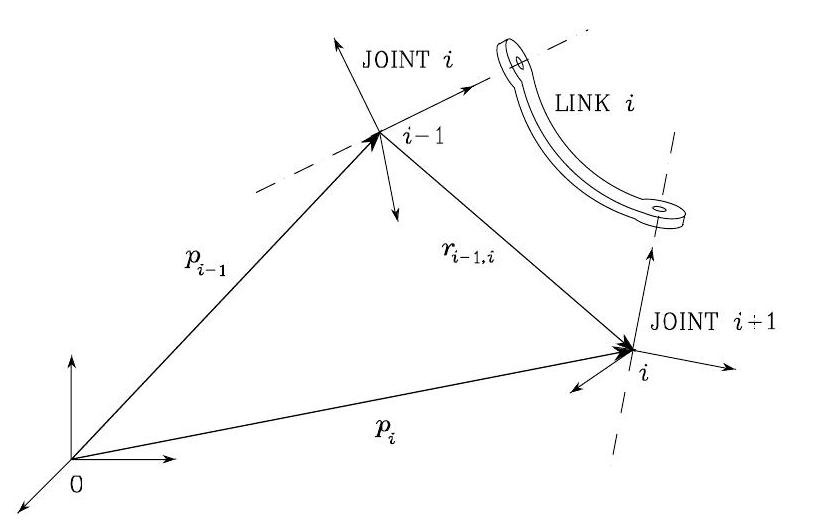
\includegraphics[max width=0.5\textwidth]{manipulator_linki}
    \caption{Characterization of generic Link $i$ of a manipulator}
    \label{fig:enter-label}
\end{figure}




\subsection{Linear Velocity}


Let $\boldsymbol{p}_{i-1}$ and $\boldsymbol{p}_{i}$ be the position of the origins of Frames $i-1$ and $i$, respectively. Also, let $\boldsymbol{r}_{i-1, i}^{i-1}$ denote the position of the origin of Frame $i$ with respect to Frame $i-1$ expressed in Frame $i-1$. 

$$
\boldsymbol{p}_{i}=\boldsymbol{p}_{i-1}+\boldsymbol{R}_{i-1} \boldsymbol{r}_{i-1, i}^{i-1}
$$

Based on the derivative of pose transformation, we have

$$
    \dot{\boldsymbol{p}}_{i}=\dot{\boldsymbol{p}}_{i-1}+\boldsymbol{R}_{i-1} \dot{\boldsymbol{r}}_{i-1, i}^{i-1}+\boldsymbol{\omega}_{i-1} \times \boldsymbol{R}_{i-1} \boldsymbol{r}_{i-1, i}^{i-1}=\dot{\boldsymbol{p}}_{i-1}+\boldsymbol{v}_{i-1, i}+\omega_{i-1} \times \boldsymbol{r}_{i-1, i}
    $$

which gives the linear velocity of Link $i$ as a function of the translational and rotational velocities of Link $i-1$.

\subsection{Angular Velocity}

Since

$$
\boldsymbol{R}_{i}=\boldsymbol{R}_{i-1} \boldsymbol{R}_{i}^{i-1}
$$

Its time derivative

$$
\boldsymbol{S}\left(\boldsymbol{\omega}_{i}\right) \boldsymbol{R}_{i}=\boldsymbol{S}\left(\boldsymbol{\omega}_{i-1}\right) \boldsymbol{R}_{i}+\boldsymbol{R}_{i-1} \boldsymbol{S}\left(\boldsymbol{\omega}_{i-1, i}^{i-1}\right) \boldsymbol{R}_{i}^{i-1}
$$

where $\boldsymbol{\omega}_{i-1, i}^{i-1}$ denotes the angular velocity of Frame $i$ with respect to Frame $i-1$ expressed in Frame $i-1$. The second term on the right-hand side  can be rewritten as

$$
   \boldsymbol{R}_{i-1} \boldsymbol{S}\left(\boldsymbol{\omega}_{i-1, i}^{i-1}\right) \boldsymbol{R}_{i}^{i-1}=\boldsymbol{R}_{i-1} \boldsymbol{S}\left(\boldsymbol{\omega}_{i-1, i}^{i-1}\right) \boldsymbol{R}_{i-1}^{T} \boldsymbol{R}_{i-1} \boldsymbol{R}_{i}^{i-1}=\boldsymbol{S}\left(\boldsymbol{R}_{i-1} \boldsymbol{\omega}_{i-1, i}^{i-1}\right) \boldsymbol{R}_{i}
   $$

   
by recalling the property of the skew-symmetric matrix. Then,

$$
\boldsymbol{S}\left(\boldsymbol{\omega}_{i}\right) \boldsymbol{R}_{i}=\boldsymbol{S}\left(\boldsymbol{\omega}_{i-1}\right) \boldsymbol{R}_{i}+\boldsymbol{S}\left(\boldsymbol{R}_{i-1} \boldsymbol{\omega}_{i-1, i}^{i-1}\right) \boldsymbol{R}_{i}
$$

leading to 

$$
    \boldsymbol{\omega}_{i}=\boldsymbol{\omega}_{i-1}+\boldsymbol{R}_{i-1} \boldsymbol{\omega}_{i-1, i}^{i-1}=\boldsymbol{\omega}_{i-1}+\boldsymbol{\omega}_{i-1, i}
    $$

which gives the expression of the angular velocity of Link $i$ as a function of the angular velocities of Link $i-1$ and of Link $i$ with respect to Link $i-1$.



\subsection{Summary}
Considering different types of Joint $i$, according to the above derivative of linear velocity and angular velocity, we have the following conclusions.


\textbf{If Joint $i$ is prismatic }

$$
\begin{aligned}
\boldsymbol{\omega}_{i} & =\boldsymbol{\omega}_{i-1} \\
\dot{\boldsymbol{p}}_{i} & =\dot{\boldsymbol{p}}_{i-1}+\dot{d}_{i} \boldsymbol{z}_{i-1}+\boldsymbol{\omega}_{i} \times \boldsymbol{r}_{i-1, i}
\end{aligned}
$$

\textbf{If Joint $i$ is revolute}

$$
\begin{aligned}
\boldsymbol{\omega}_{i} & =\boldsymbol{\omega}_{i-1}+\dot{\vartheta}_{i} \boldsymbol{z}_{i-1} \\
\dot{\boldsymbol{p}}_{i} & =\dot{\boldsymbol{p}}_{i-1}+\boldsymbol{\omega}_{i} \times \boldsymbol{r}_{i-1, i}
\end{aligned}
$$







\end{document}